%! Author = joels
%! Date = 05/01/2021

\section{GUI-Programmierung}
\subsection{XAML Allgemein}
Beschreibungssprache von Microsoft zur Gestaltung graphischer Oberflächen.\\
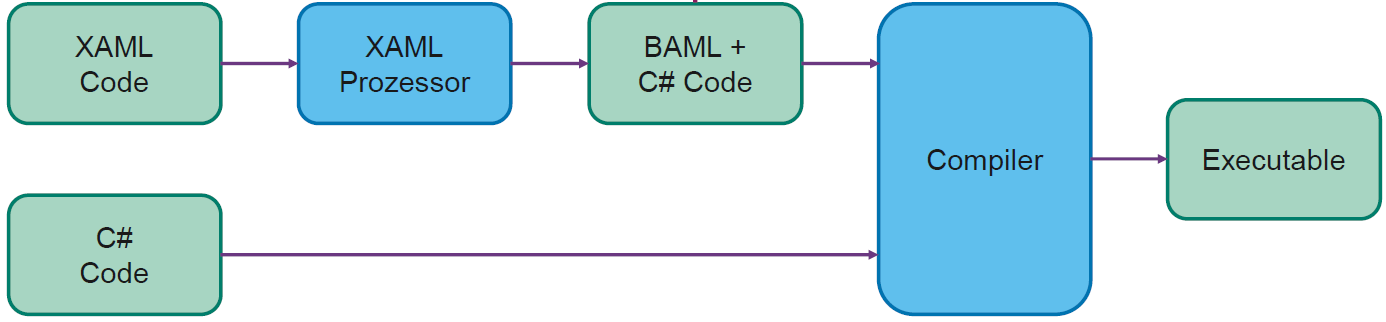
\includegraphics{xaml.png}
Für Design kann auch C\# verwendet werden, XAML ist jedoch leichter, kürzer, lesbarer und hat einen Designer. Microsoft Blend für das Designen.
\subsubsection{Visual Tree und Logical Tree}
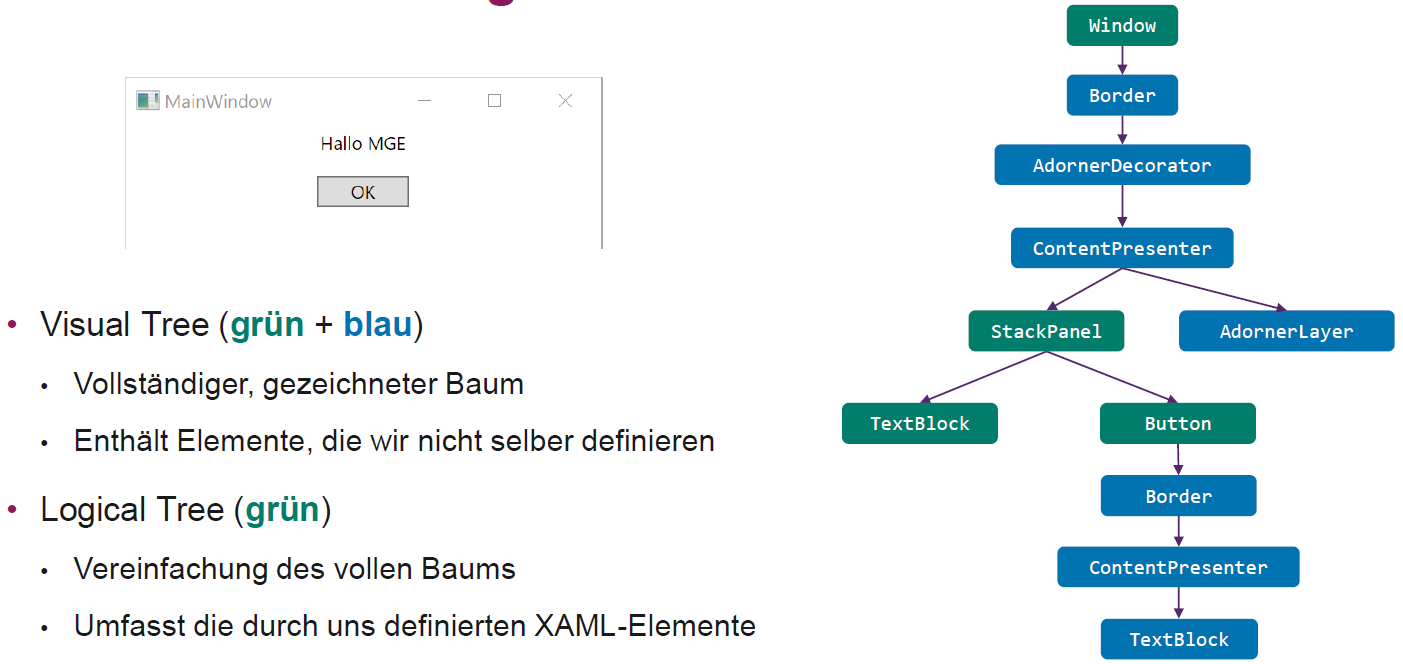
\includegraphics{xaml_tree.png}
\subsubsection{Namespaces}
\textbf{Mit xmlns werden XML-Namespaces definiert.}\\
$\rightarrow$ Ohne Doppelpunkt: \textcolor{blue}{Standard-Namespace} (Elemente können ohne Präfix verwendet werden)\\
$\rightarrow$ Mit Doppelpunkt: \textcolor{blue}{Nenannter Namespace} (Elemente können nur mit Präfix verwendet werden)\\
\textbf{\textcolor{blue}{Übliche Namespaces in WPF:}}
\begin{itemize}[topsep=0pt, leftmargin=4mm]
    \setlength\itemsep{-0.3em}
    \item Der Standard-Namespace wird auf die WPF Control Library gesetzt
    \item x für XAML-spezifische Elemente
    \item d für Elemente des visuellen Designers
    \item mc für Elemente der «Markup Kompatibilität»
    \item local für Elemente aus unserem eigenen Assembly
\end{itemize}
\begin{lstlisting}
<Window xmlns="http://schemas.microsoft.com/winfx/2006/xaml/presentation"
   xmlns:x="http://schemas.microsoft.com/winfx/2006/xaml"
   xmlns:d="http://schemas.microsoft.com/expression/blend/2008"
   xmlns:mc="http://schemas.openxmlformats.org/markup-compatibility/2006"
   xmlns:local="clr-namespace:Vorlesung_09"
   mc:Ignorable="d"
   ... />
\end{lstlisting}
\subsubsection{Named Elements}
\textbf{Elemente können benannt werden.} $\rightarrow$ Ermöglicht Zugriff auf Code-Behind. Attribut führt zu Property in generierter Klasse
\begin{lstlisting}
// XAML:
<TextBlock Name="WpfAttribute" Text="WPF" />
<TextBlock x:Name="XamlAttribute" Text="XAML" />
// Code Behind:
this.WpfAttribute.Text = "...";
this.XamlAttribute.Text = "...";
\end{lstlisting}
\subsubsection{Syntaxen}
\begin{lstlisting}
// Attribute Syntax:
<Button Background="Blue"
        Foreground="Red"
        Content="Mein Button" />
// Property Element Syntax:
<Button>
    <Button.Background>
        <SolidColorBrush Color="Blue"/>
    </Button.Background>
    <Button.Foreground>
        <SolidColorBrush Color="Red"/>
    </Button.Foreground>
    <Button.Content>
        Mein Button
    </Button.Content>
</Button>
\end{lstlisting}
\subsubsection{Type Converters}
\begin{lstlisting}
// XAML:
<local:LocationControl Center="10, 20" />
// Control:
public class LocationControl : TextBlock {
    public Location Center {
        set => this.Text = $"{value.Lat} / {value.Long}";
    }
}
// Model:
[TypeConverter(typeof(LocationConverter))]
public class Location {
    public double Lat { get; set; }
    public double Long { get; set; }
}
// Type Converter:
public class LocationConverter : TypeConverter {
    public override object ConvertFrom(
      ITypeDescriptorContext context,
      CultureInfo culture,
      object value) {
        //Zur Kürzung des Beispiels auf Checks verzichtet:
        // - Ist value wirklich ein string?
        // - Enthält das Array exakt 2 Elemente?
        // - Sind die strings zu double konvertierbar?
        var valueAsString = (string) value;
        var valueArray = valueAsString.Split(',');
        return new Location {
            Lat = Convert.ToDouble(valueArray[0]),
            Long = Convert.ToDouble(valueArray[1])
        };
    }
}
\end{lstlisting}
\subsubsection{Content Properties}
Jedes XAML-Element kann genau eine Eigenschaften als seinen Inhalt definieren. Einige Elemente können, neben reinem Text, auch andere Elemente enthalten.
\begin{lstlisting}
<Button Content="Label" />
<Button>Label</Button>
<Button Width="150" Height="60">
    <StackPanel>
        <TextBlock Text="Gross"
                   TextAlignment="Center"
                   FontSize="20" />
        <TextBlock Text="Und hier klein"
                   FontSize="12"
                   Foreground="#888888" />
    </StackPanel>
</Button>
\end{lstlisting}
\subsubsection{Markup Extensions}
Erlauben die Erweiterung des XAML-Markup mit zusätzlicher Logik. Die Logik wird in geschweiften Klammern platziert $\{$ ... $\}$. Verwendet bei Styling und Data Binding.
\begin{lstlisting}
// XAML:
<TextBlock Text="{local:LocationExtension Lat=10,Long=20}" />
// Marup Extension:
public class LocationExtension : MarkupExtension {
    public string Lat { get; set; }
    public string Long { get; set; }
    public override object ProvideValue(IServiceProvider s) {
        return this.Lat + " / " + this.Long;
    }
}
\end{lstlisting}
\subsubsection{Attached Properties}
Setzt Eigenschaft auf einem Element, die zu einem anderen Element gehört. Die Eigenschaft wird sozusagen einem anderen Element angehängt.
\begin{lstlisting}
<Grid>
    <Grid.RowDefinitions>
        <RowDefinition Height="30" />
        <RowDefinition Height="20" />
        <RowDefinition Height="10" />
    </Grid.RowDefinitions>

    <TextBlock Grid.Row="0" Name="G" Background="Green" />
    <TextBlock Grid.Row="1" Name="R" Background="Red" />
    <TextBlock Grid.Row="2" Name="B" Background="Blue" />
</Grid>
\end{lstlisting}
\subsection{Grundelemente}
\subsubsection{Klassenhierarchie}
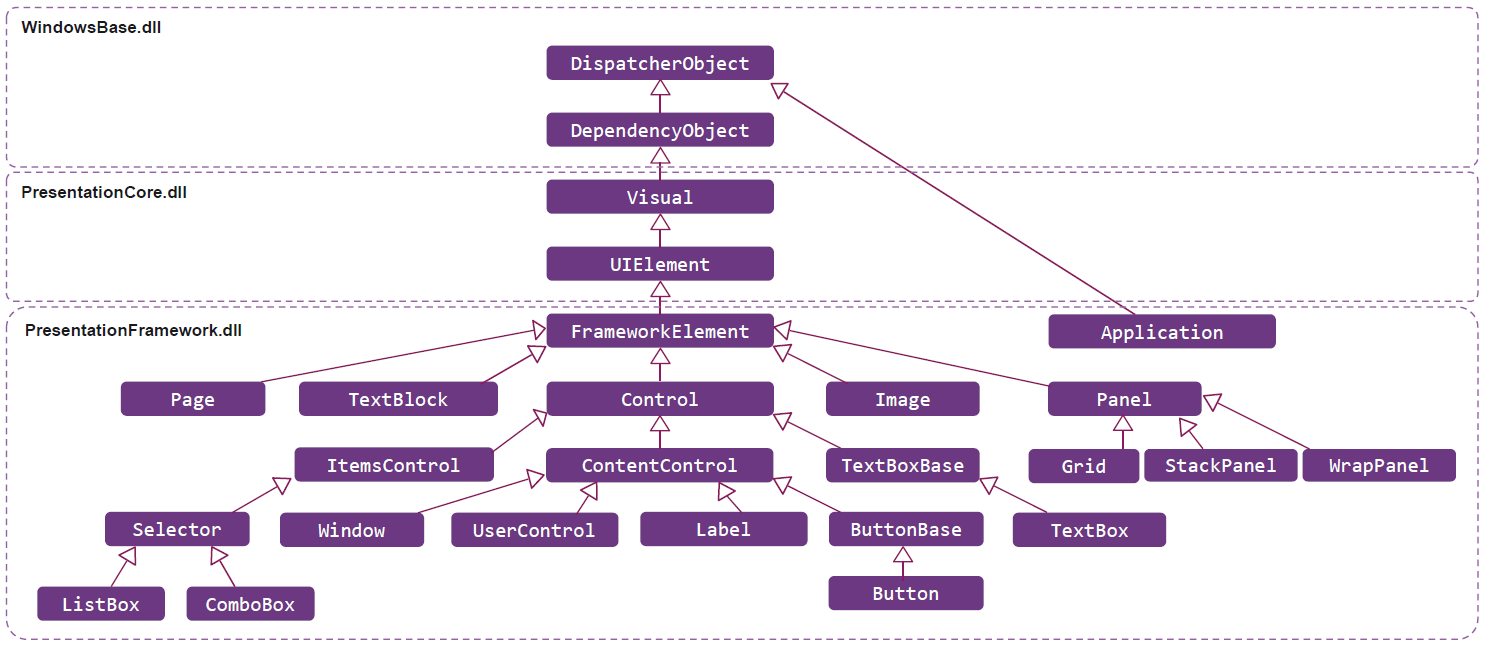
\includegraphics{klassenhierarchie.png}
\subsubsection{Application}
\textbf{Einstiegspunkt in die Anwendung.} Main()-Methode in generiertem Code. Erzeugt Application-Instanz. Definiert via StartupUri die erste View.
\begin{lstlisting}
// XAML:
<Application x:Class="Vorlesung_09.App"
    StartupUri="MainWindow.xaml">
</Application>
// Code Behind:
public partial class App : Application{ }
// Generated Code:
// Nur ein Auszug
public partial class App : System.Windows.Application {
    public void InitializeComponent() {
        this.StartupUri = new System.Uri("MainWindow.xaml", System.UriKind.Relative);
    }
    public static void Main() {
        Vorlesung_09.App app = new Vorlesung_09.App();
        app.InitializeComponent();
        app.Run();
    }
}
\end{lstlisting}
\subsubsection{Window - Sichtbare Elemente}
\begin{center}
    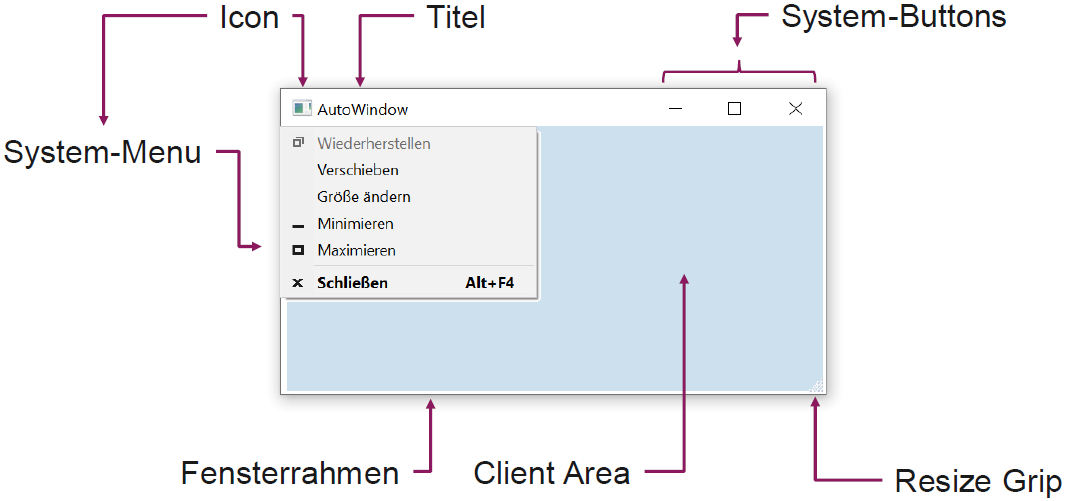
\includegraphics[width=0.8\linewidth]{window.png}
\end{center}
\subsubsection{Window - Wichtige Eigenschaften}
\begin{itemize}[topsep=0pt, leftmargin=4mm]
    \setlength\itemsep{-0.3em}
    \item Title – Name des Fensters
    \item Icon – Icon des Fensters
    \begin{itemize}[topsep=0pt, leftmargin=4mm]
        \setlength\itemsep{-0.3em}
        \item Bild mit Build Action \dq Resource\dq hinzufügen
        \item Verschiedene Dateiformate unterstützt
    \end{itemize}
    \item ShowInTaskbar – Sichtbarkeit in Taskleiste
    \item WindowStyle – Aussehen des Fensters
    \item WindowStartupLocation – Anzeigeposition
    \item ResizeMode – Modus zur Grössenänderung
\end{itemize}
\subsubsection{UIElement}
\textbf{Wichtigste Basisklasse für visuelle WPF-Elemente.}\\
Definiert grundlegende Elemente, Methoden und Events:\\
\textcolor{blue}{IsEnabled:} Reagiert das Element auf Interaktionen?\\
\textcolor{blue}{IsFocused:} Ist das Element gerade aktiv?\\
\textcolor{blue}{Visibility:} Ist das Element sichtbar? $\rightarrow$ z.B. Collapsed (Unsichtbar, keinen Platz), Hidden (Unsichtbar, belegt Platz), Visible (Sichtbar), etc.
\subsubsection{FrameworkElement}
Erweitert UIElement um zusätzliche Funktionalität, unter anderem:
\begin{itemize}[topsep=0pt, leftmargin=4mm]
    \setlength\itemsep{-0.3em}
    \item Name-Property für Zugriff
    \item Logical Tree
    \item Layout System
    \item Visuelles Styling (Woche 10)
    \item Data Binding (Woche 11)
\end{itemize}
\textbf{\textcolor{blue}{Grössenangaben:}}\\
Width, Height und Margin, Kein Padding. Zusätzlich MinWidth, MaxWidth und MinHeight, MaxHeight.\\
\textbf{\textcolor{blue}{Dimensionen:}}\\
Auto: Automatische Grösse (wrap\_content)\\
px: Device Independent Pixels, 1in == 96px\\
\textbf{\textcolor{blue}{Ausrichtungen:}}\\
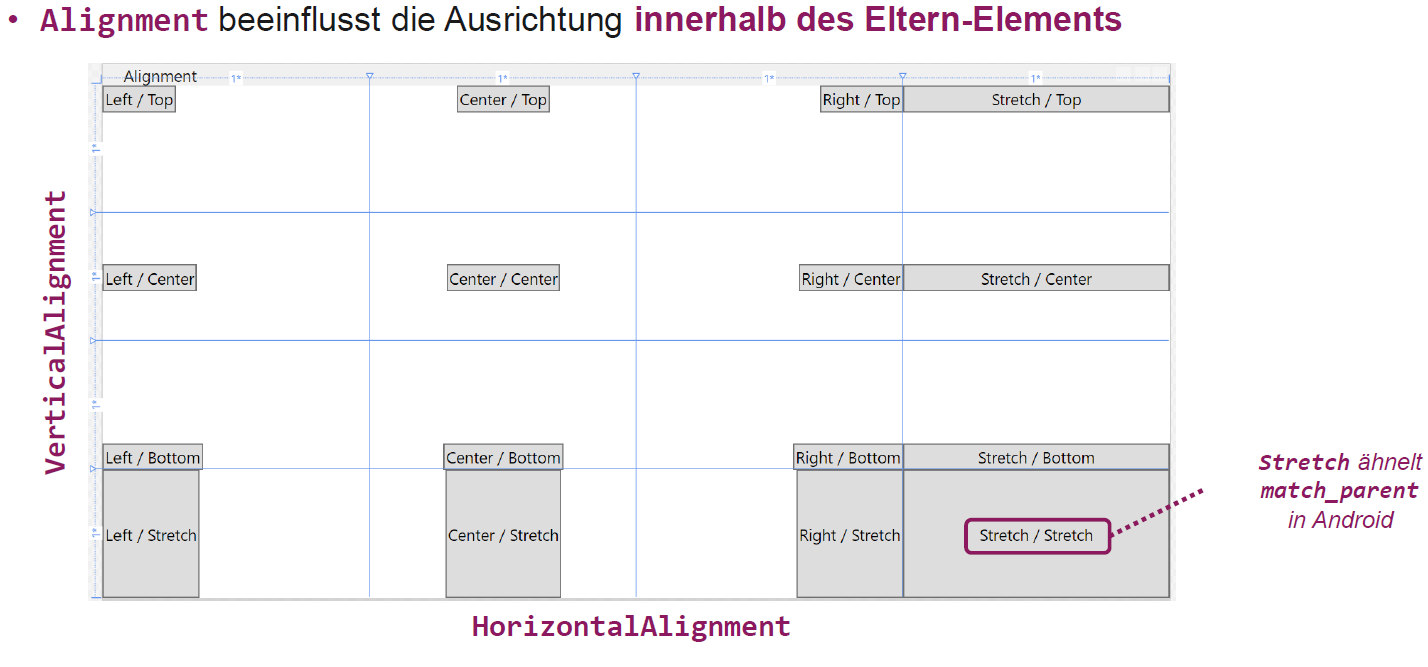
\includegraphics{alignment.png}
\subsubsection{Control}
\textbf{Basis-Klasse für Controls mit Benutzerinteraktion.}\\
Erweitert FrameworkElement um zusätzliche Funktionalität: Gestaltungsmöglichkeiten (Farben, Schriften, Ränder), Ausrichtungen der Kind-Elemente, Control Templates (Woche 10)\\
\textbf{\textcolor{blue}{Rahmen/Ränder:}}\\
Neue Eigenschaften: \textcolor{blue}{padding} (Innenabstand), \textcolor{blue}{BorderThickness} (Rahmenstärker), \textcolor{blue}{CornerRadius} (Radius für abgerundete Ecken)\\
Grössenangaben für Margin und Padding:\\
\textbf{n} - Selber Wert für alle Seiten\\
\textbf{x,y} - X für Horizontal, Y für Vertikal\\
\textbf{l,t,r,b} - Links, Oben, Rechts, Unten\\
\textbf{\textcolor{blue}{Ausrichtung:}}
\begin{center}
    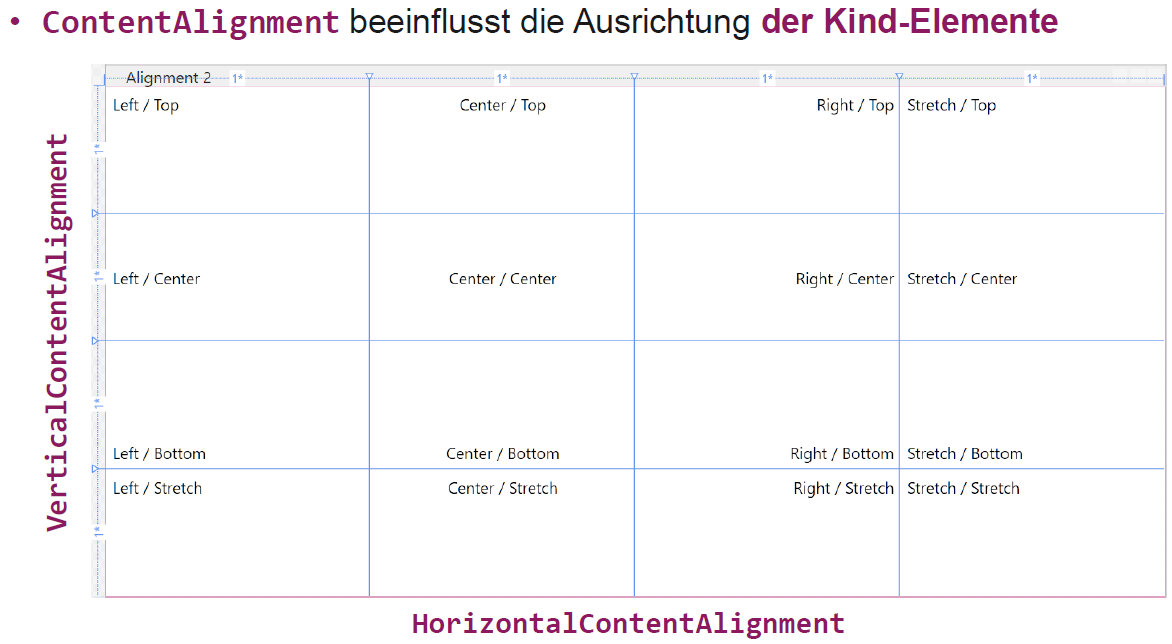
\includegraphics[width=0.85\linewidth]{content_alignment.png}
\end{center}
\textbf{\textcolor{blue}{Farben/Schriften:}}\\
Farbgebung mit Brushes (\dq Pinsel\dq): Foreground, Background, BorderBrush\\
Schriftbild: FontFamily, FontSize, FontStretch, FontStyle, FontWeight

\subsection{Layouts}
Layouts sind Container für Kind-Elemente. Haben eine Parent-Child Beziehung. Verschachtelung ist möglich.\\
\textbf{Verfügbare Layouts in WPF:}
\begin{itemize}[topsep=0pt, leftmargin=4mm]
    \setlength\itemsep{-0.3em}
    \item StackPanel – Horizontale oder vertikale Auflistung
    \item WrapPanel – Wie Stack, aber mit Zeilen-/Spaltenumbruch
    \item DockPanel – Kinder werden an Seiten/im Zentrum \dq angedockt\dq
    \item Grid – Kinder werden den Zellen einer Tabelle zugeordnet
\end{itemize}
\subsubsection{StackPanel}
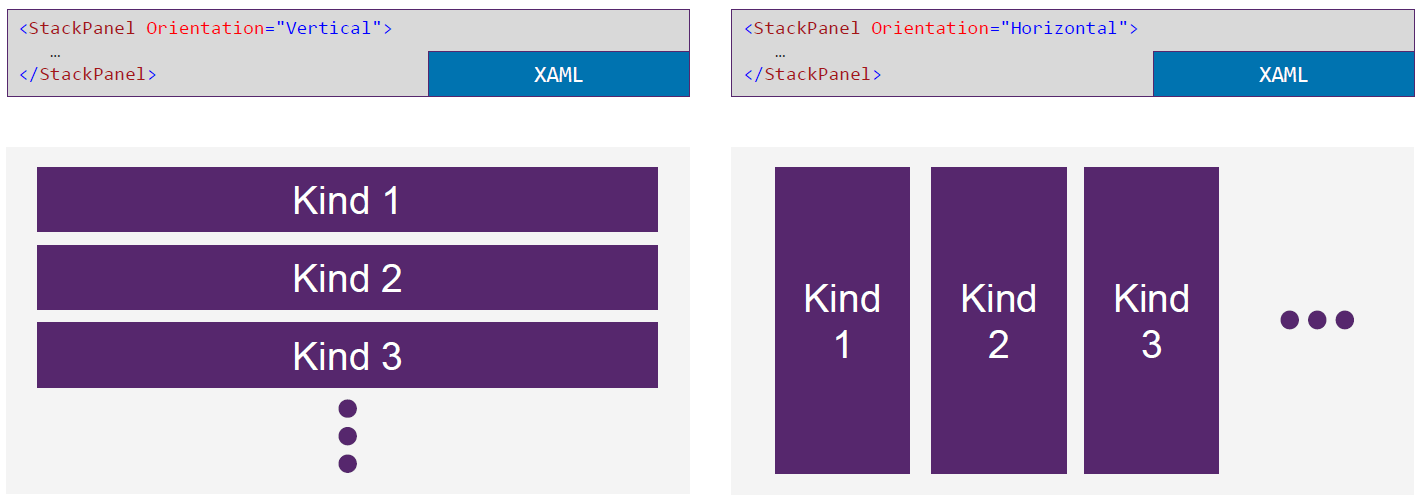
\includegraphics{stack_panel.png}
\subsubsection{WrapPanel}
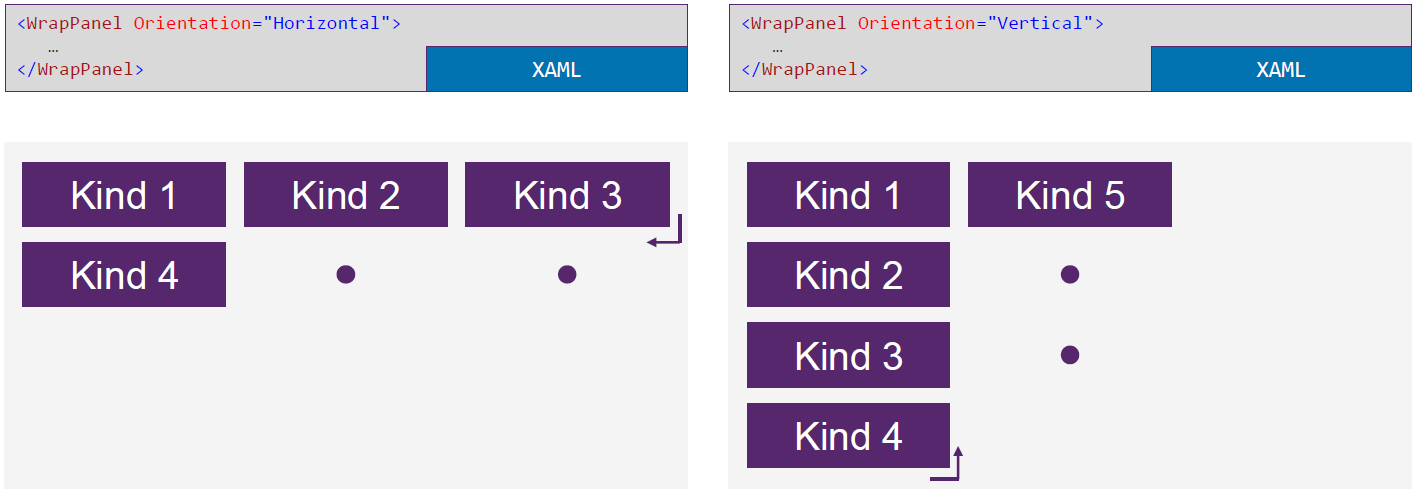
\includegraphics{wrap_panel.png}
\subsubsection{DockPanel}
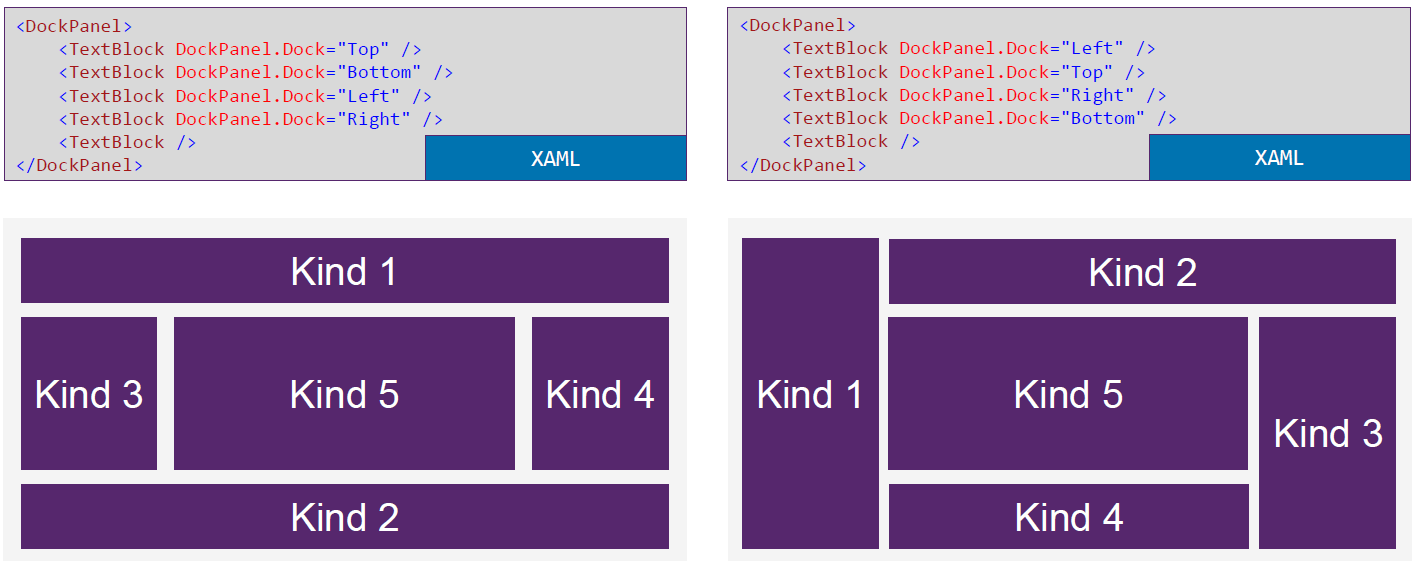
\includegraphics{dock_panel.png}\\
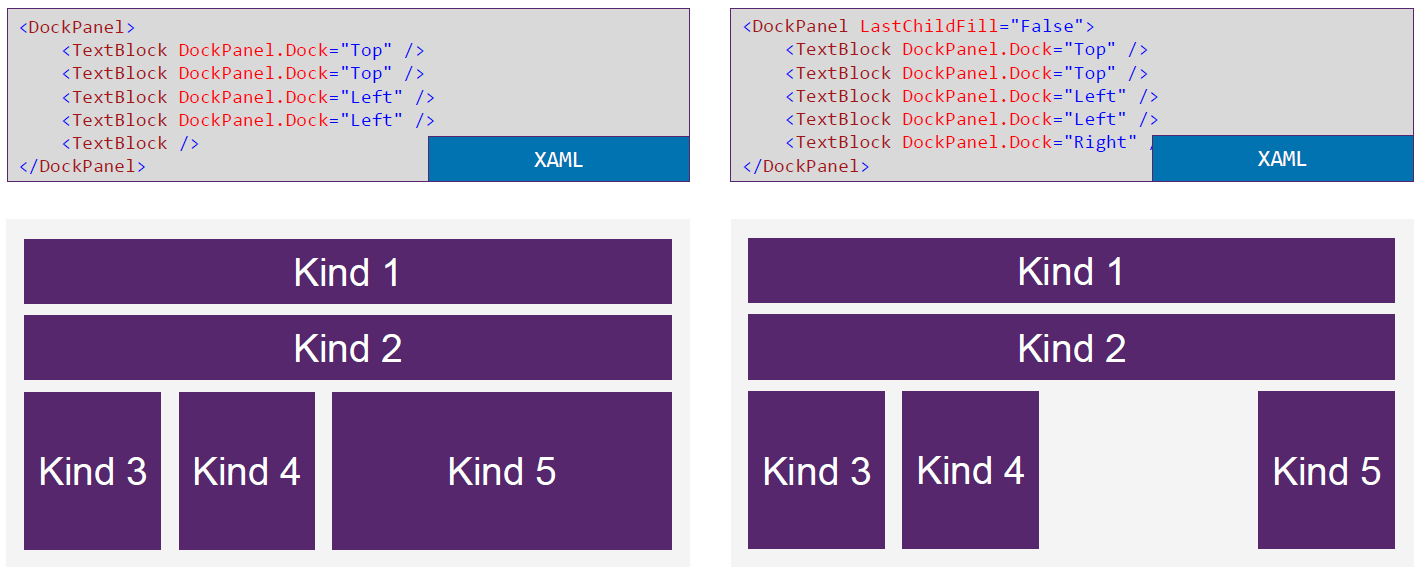
\includegraphics{dock_panel_2.png}
\subsubsection{Grid}
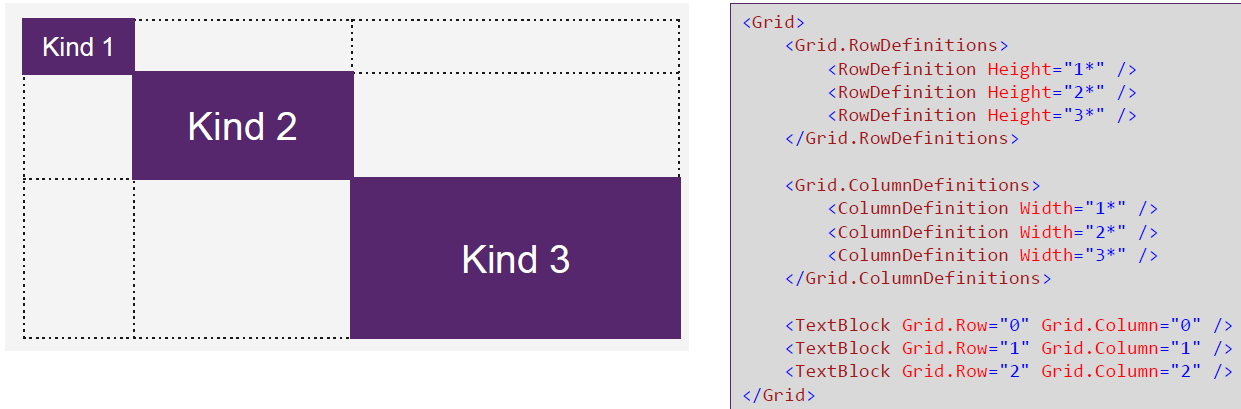
\includegraphics{grid.png}\\
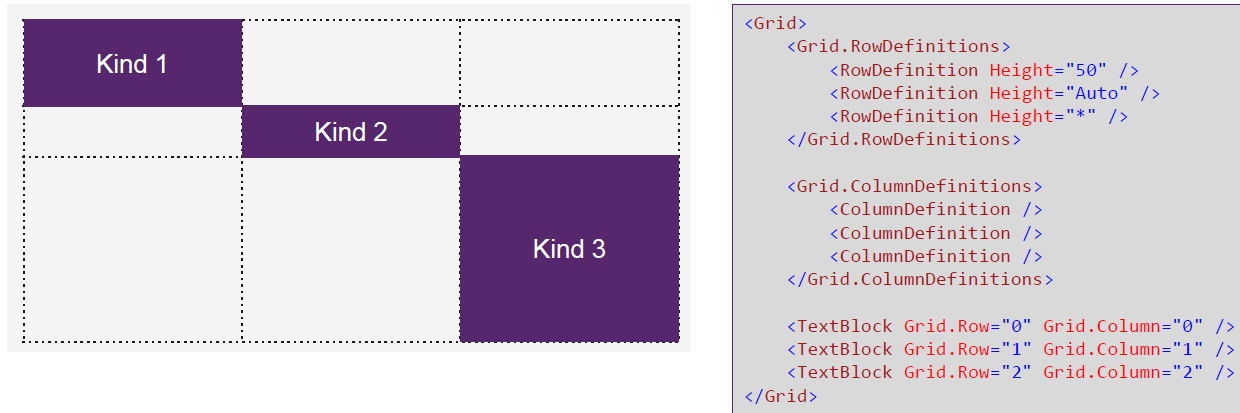
\includegraphics{grid_2.png}